\chapter{Model Development}\label{chapter:model_development}
This chapter contains take-off performance assessment at several levels of fidelity. Originally, there were supposed to be three levels of fidelity. However, due to uncertainty around the models that were supposed to comprise the level 3 assessment, it was decided to use the level 2 model. This section first details some general take-off performance modeling and afterwards continues to describe the level-I and level-II models. A flowchart with an overview of the models and their respective characteristics is given in \autoref{fig:flowchart_models}. The effects in green have not yet been included in the analysis: in other words, model level 3 has not yet been developed.

\begin{figure}[!ht]
    \centering
    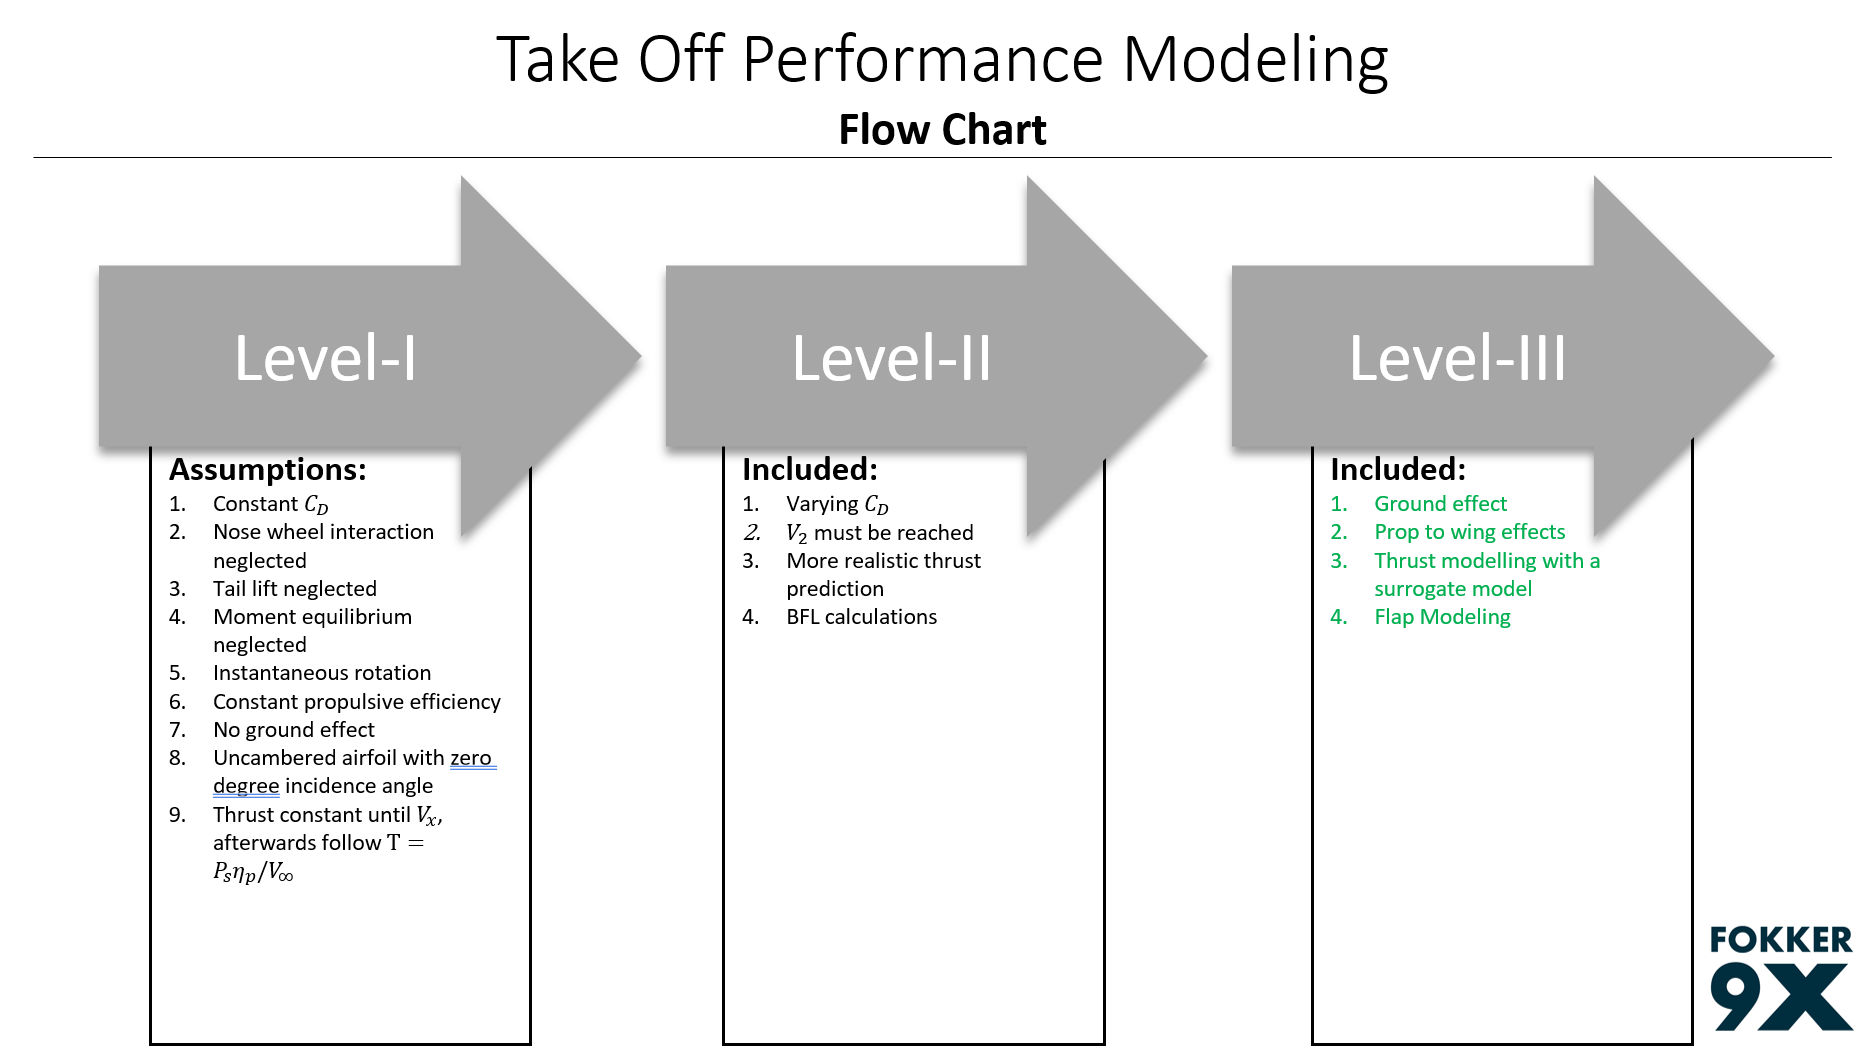
\includegraphics[width=\linewidth]{figures/program_flowchart.png}
    \caption{Flowchart of take-off models}
    \label{fig:flowchart_models}
\end{figure}

\section{Take-Off Modeling Strategy}\label{sec:generalTO}
Take-off is divided into two phases; the ground- and airborne-phase. The ground phase occurs when the aircraft is not airborne yet. A schematic of the forces in the ground phase is given in \autoref{fig:groundphase_schematic}, and the schematic of the airborne phase in \autoref{fig:airbornephase_schematic}. All models are based on the same set of equations, given by Equations~\eqref{eq:equillibrium_forcex} \textemdash\;\eqref{eq:equillibrium_moment}. The friction coefficient goes to zero in the aforementioned equations when the lift becomes larger than the weight. Also, the angle of attack, $\alpha$ is simply zero during the ground phase, thus equating $\cos$ and $\sin$ to one and zero, respectively. Furthermore, it is important to note that the moment equilibrium is not satisfied, since the nose-wheel is neglected, and it is assumed that all forces act from the same point.

\begin{figure}[!ht]
    \centering
    \begin{minipage}{.48\textwidth}
      \centering
      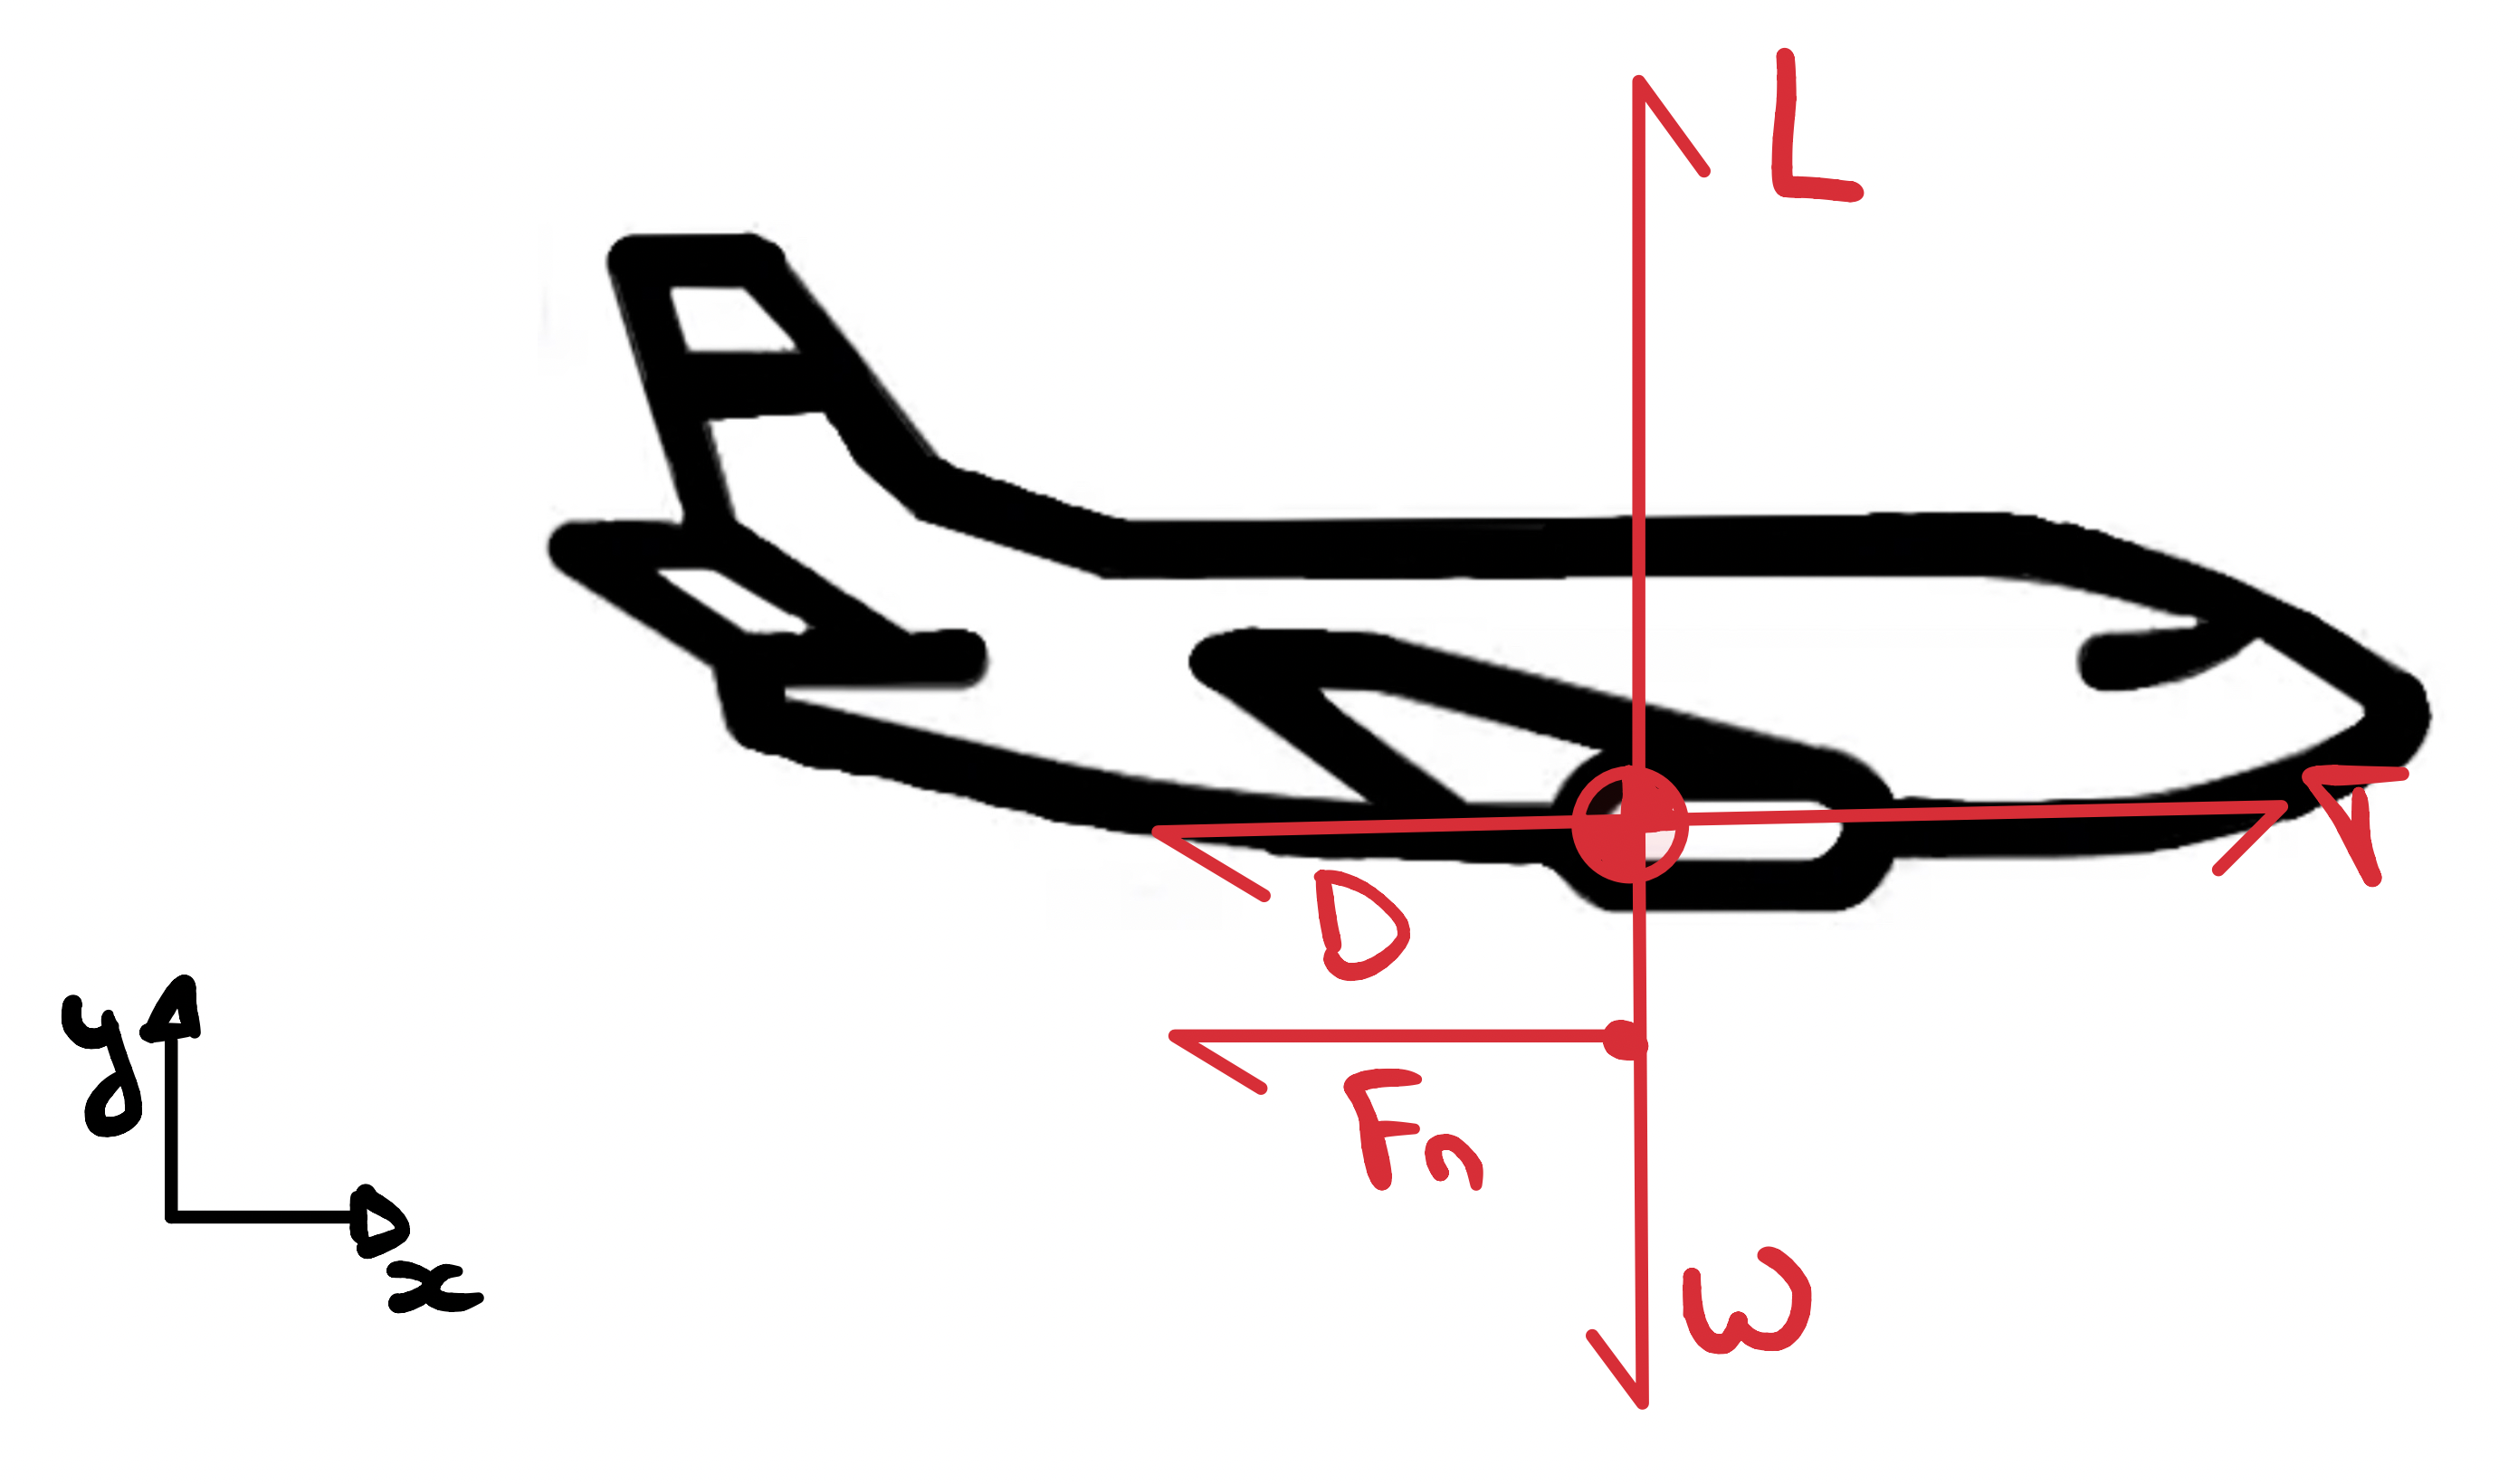
\includegraphics[width=\linewidth]{figures/schematic_groundphase.png}
      \captionof{figure}{Schematic of forces during the ground phase during take-off}
      \label{fig:groundphase_schematic}
    \end{minipage}%
    \hfill
    \begin{minipage}{.48\textwidth}
      \centering
      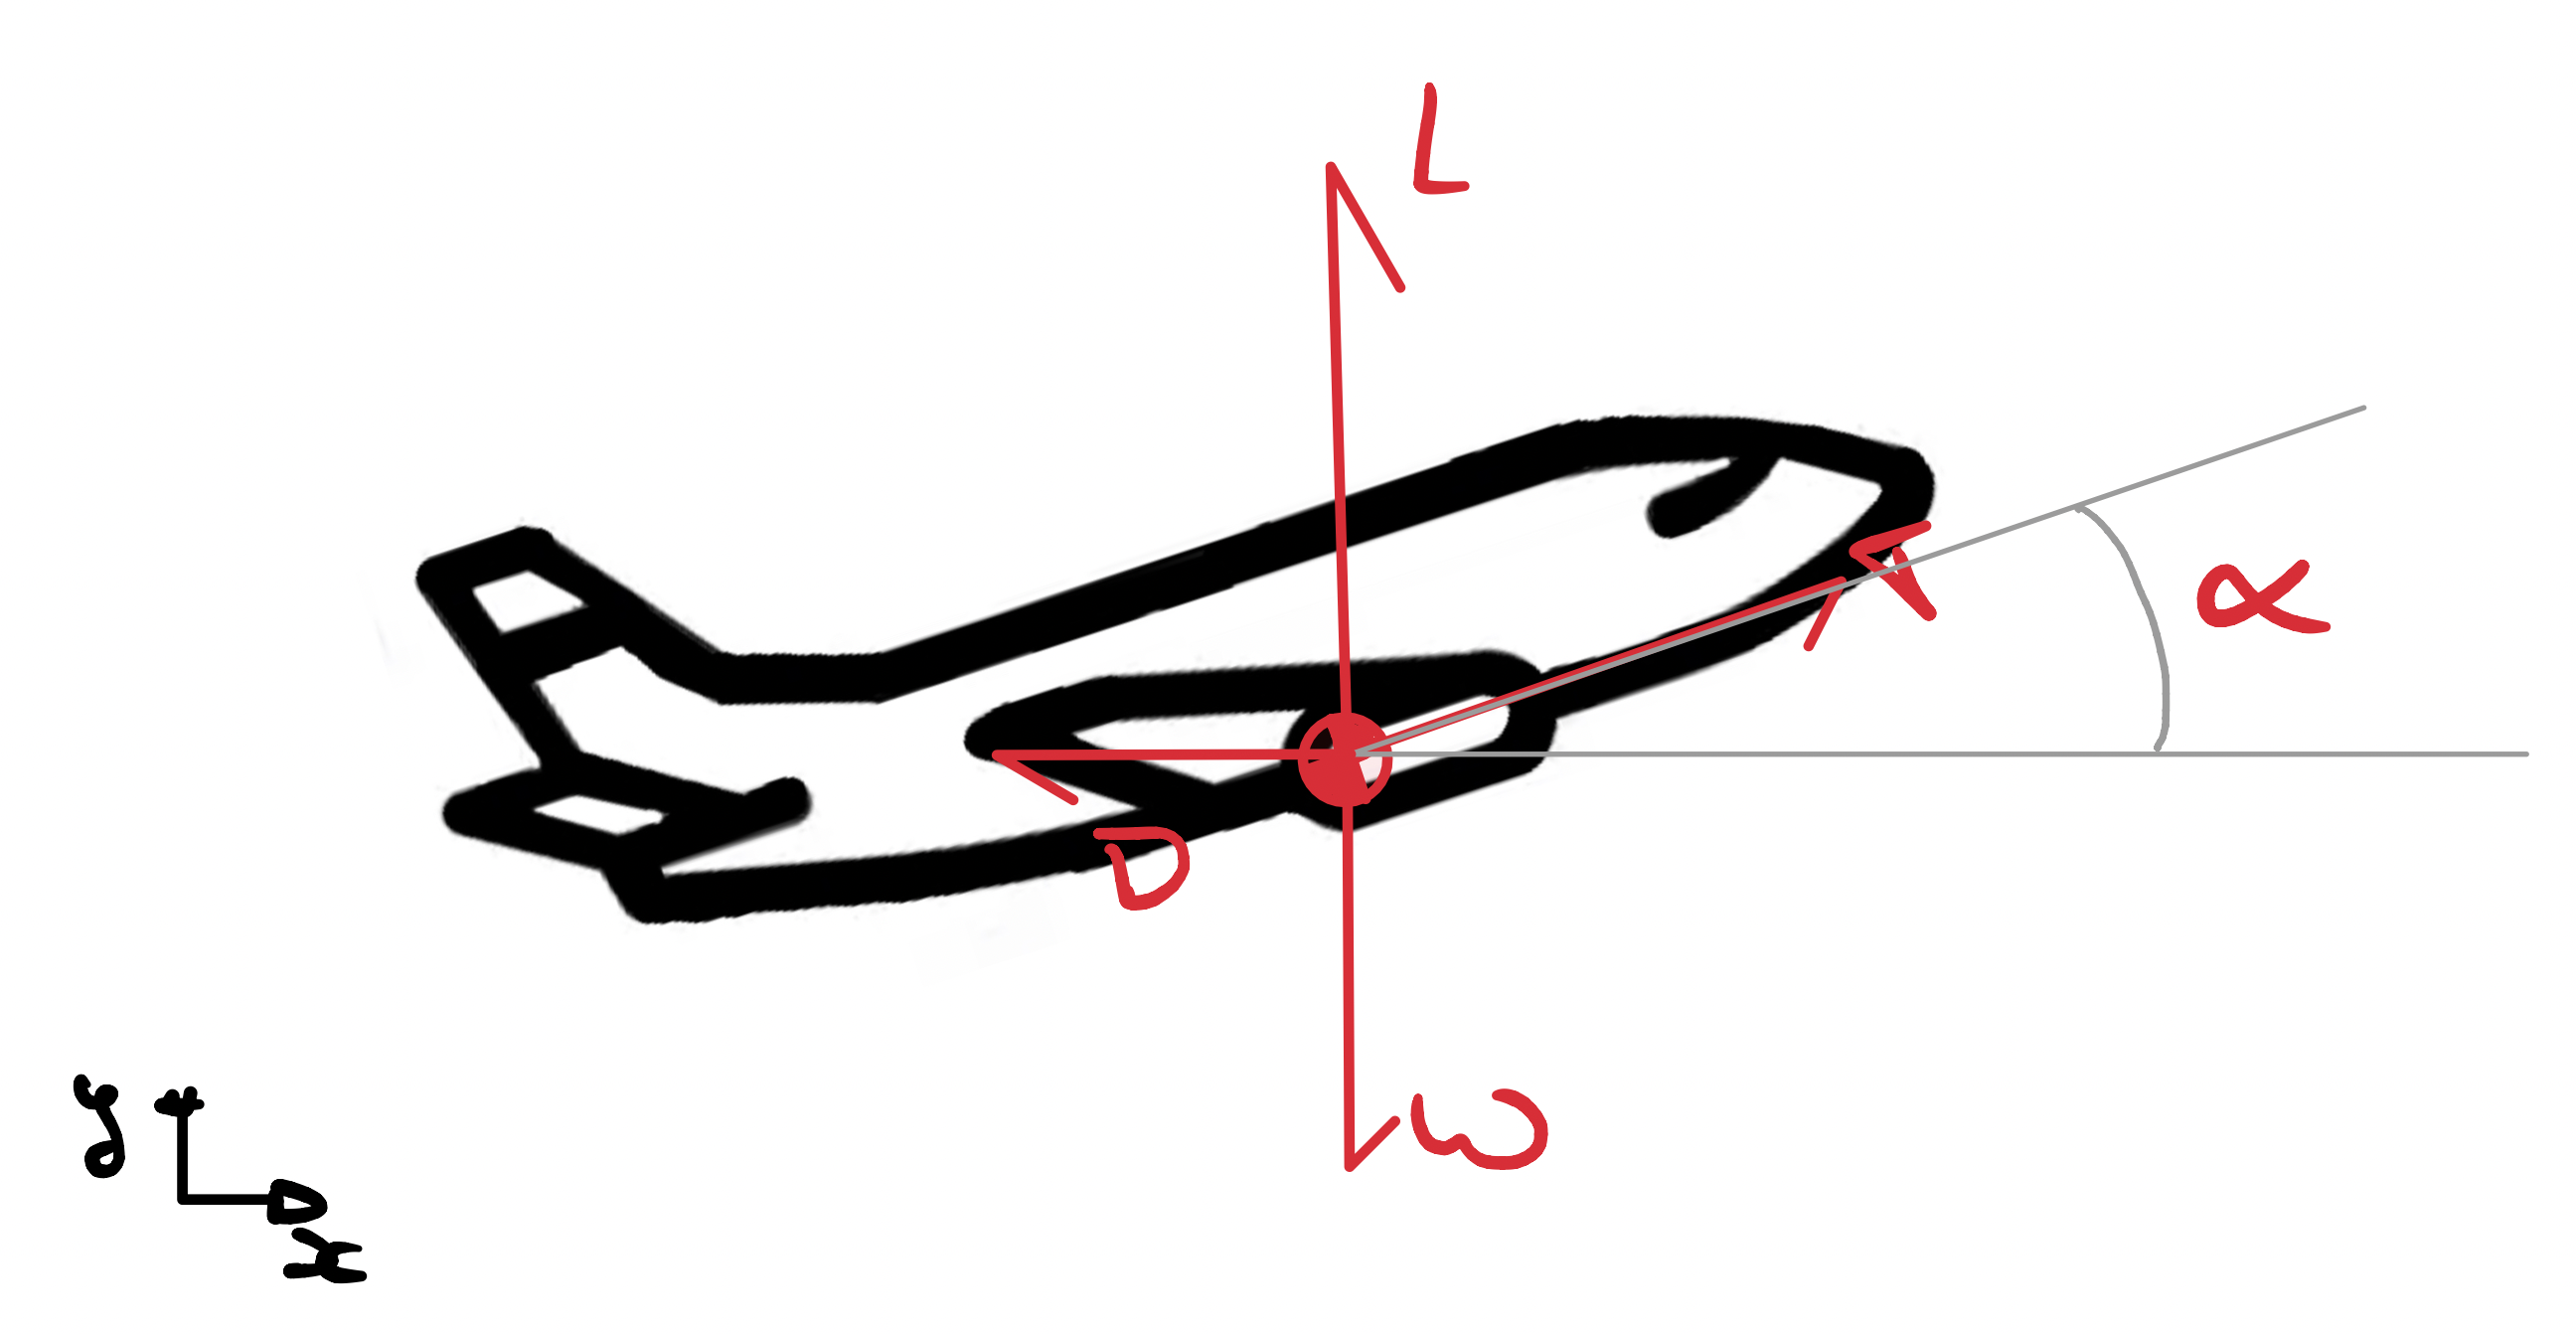
\includegraphics[width=\linewidth]{figures/schematic_airbornephase.png}
      \captionof{figure}{Schematic of forces during the airborne phase during take-off}
      \label{fig:airbornephase_schematic}
    \end{minipage}
\end{figure}

\begin{equation}
    \label{eq:equillibrium_forcex}
    \sum F_x: T(V_\infty)\cdot \cos{(\alpha)} - D(V_\infty) - F_n(V_\infty) = m a_x
\end{equation}

\begin{equation}
    \label{eq:equillibrium_forcey}
    \sum F_y: T(V_\infty)\cdot \sin{(\alpha)} + L(V_\infty) - W = m a_y
\end{equation}

\begin{equation}
    \label{eq:equillibrium_moment}
    \sum M_{c.g.}: F_n \cdot y_{c.g.}-y_\text{l.g.} != 0
\end{equation}

For aircraft design purposes it is useful to express these equations in terms of $W/S$ and $T/W$. Therefore, Equations~\eqref{eq:equillibrium_forcex_WS_TW}\textemdash\eqref{eq:equillibrium_forcey_WS_TW} give the force equilibrium equations in terms of $W/S$ and $T/W$.

\begin{equation}
    \label{eq:equillibrium_forcex_WS_TW}
    \frac{T}{W}\frac{W}{S}\frac{1}{q} \cos{(\alpha+\gamma)}-C_D\cos{(\gamma)}-C_L\sin{(\gamma)}-F_n \frac{1}{qS} = \frac{W}{S}\frac{1}{q g} \frac{dV_x}{dt}
\end{equation}

\begin{equation}
    \label{eq:equillibrium_forcey_WS_TW}
    \frac{T}{W}\frac{W}{S}\frac{1}{q} \sin{(\alpha+\gamma)}-\frac{W}{S}\frac{1}{q} - C_D\sin{(\gamma)}+C_L\cos{(\gamma)} = \frac{W}{S}\frac{1}{q g} \frac{dV_y}{dt}
\end{equation}

In the aforementioned equations, thrust, drag, lift and the friction force are given by the equations below:\newline

\noindent\begin{minipage}{.5\linewidth}
    \begin{equation}
        \label{eq:thrust}
        T(V_\infty) = \frac{\eta_p P_s}{V_\infty} 
    \end{equation}
\end{minipage}%
\begin{minipage}{.5\linewidth}
    \begin{equation}
        \label{eq:lift}
        L(V_\infty) = 0.5 \rho V_\infty^2 S C_{L}
    \end{equation}
\end{minipage}\newline
\noindent\begin{minipage}{.5\linewidth}
    \begin{equation}
        \label{eq:drag}
        D(V_\infty) = 0.5 \rho V_\infty^2 S C_{D}
    \end{equation}
\end{minipage}%
\begin{minipage}{.5\linewidth}
    \begin{equation}
        \label{eq:friction}
        F_n(V_\infty) = (W-L) \cdot \mu
    \end{equation}
\end{minipage}\newline

The modeling approach discretises the take-off maneuver in infinitesimal small time steps and calculates the next state based on the current forces, and thus accelerations. The advantage of this approach is that po0licies, such as rotation, can be controlled and that all information is saved at each time-step.

Deceleration modelling...

he simulation parameters are given in \autoref{tab:simulationparams}. The stall speed was determined by assuming $C_{L,flaps,max}$, listed in \autoref{tab:simulationparams}, and calculating the speed using Equation \eqref{eq:lift}. As of now it is vague whether you're allowed to use flaps to determine this speed but for the moment this is assumed to be correct.\\

Reach V2min at h2...\\

\begin{table}[!ht]
    \centering
    \begin{tabular}{cccc}\hline \hline
        \textbf{Parameter}          & \textbf{Symbol}       & \textbf{Value}                         & \textbf{Unit} \\ \hline
        Lift Coefficient            & $C_L$                 & 0.5                                    & -             \\
        Max Lift Coefficient Clean  & $C_{L,clean,max}$     & 1.5                                    & -             \\
        Max Lift Coefficient Flaps  & $C_{L,flaps,max}$     & 1.8~2.1                                & -             \\
        Drag Coefficient            & $C_{D,0}$             & 0.025                                  & -             \\
        Friction Coefficient        & $\mu$                 & 0.02~\cite{torenbeek2013synthesis}     & -             \\
        Air Density                 & $\rho$                & 1.225                                  & $kg/m^3$      \\
        Propulsive Efficiency       & $\eta_p$              & 0.85                                   & -             \\
        Climb angle                 & $\alpha_\text{climb}$ & 10                                      & deg           \\
        Rotation time               & $s_r$                 & 4                                      & $s$           \\
        Stall speed                 & $V_s$                 & 32.4                                   & $m/s$         \\
        Rotation speed              & $V_r$                 & 4                                      & $s$           \\ \hline
    \end{tabular}
    \caption{Simulation parameters}
    \label{tab:simulationparams}
\end{table}

\subsection{Solving Strategy}
Constraining at Vlof...

\subsection{Rotation Strategy}\label{sec:rotation}
The rotation strategy, starting at $V_r$, is crucial in reaching the required $V_2$, and decreasing the take-off distance. During the project, a more sophisticated specific energy power (SEP) based strategy was considered to directly determine how much of the excess power is delegated to kinetic and potential energy. Eventually it was found that this strategy was rather convoluted since the goal became to create a realistic aircraft pitch profile. Therefore, the pitch was controlled directly. The question remains 'what rotation strategy returns the shortest take-off distance?'. The limiting case would be to instantly rotate the aircraft to 90 degrees and all horizontal speed into vertical speed - without horizontal velocity the take-off distance won't increase. Obviously, this isn't a desirable or feasible rotation strategy for a commercial aircraft. The other extreme is to not rotate after $V_{lof}$. In the latter scenario, the aircraft will reach $h_{screen}$ with a high $V_2$ and $s_{tofl}$. It can be concluded that the solution lies somewhere in between. Another factor to take into account is that pilots are not (yet) computers, so they cannot execute a very specific rotation strategy. With these three considerations, it was determined to use a simple linearly increasing angle of attack, assuming the $3\;deg/s$ given by Torenbeek~\cite{torenbeek2013synthesis} as a typical rotation speed, until the climb angle (defined by the user) is reached, at that point the angle of attack (not pitch!) will remain constant.

\section{Wing Systems Modelling}

\subsection{Clean Wing Modelling}
Lift...\\
Drag...

\subsection{Flap Modelling}
Lift...\\
Drag...

\subsection{Propeller Induced Lift and Drag Modelling}
Blown-wing effects can be included by including the models described by Reynard de Vries~\cite{de2019preliminary}. His work includes formula that describe how the $C_L$ and $C_D$ of a wing change due to the propellers being configured in a tractor configuration. The model uses those equations, given below. It should be pretty straightforward to figure out how the model works, and otherwise the code explains it.

\subsection{Ground Effect Modelling}
The ground effect is interesting to model, since it substantially affects wing performance. Luckily, Torenbeek came up with some nifty equations, which essentially make the whole process plug and play. It is important to beware of the denotations, which can be found in pages 551-553. The method will not be explained here any further because the book essentially describes the exact same procedure. The difference between level-II and level-III drag- and lift-coefficients are shown in \autoref{fig:drag_level2_3} and \autoref{fig:lift_level2_3}, respectively.

\begin{figure}[!ht]
    \centering
    \begin{minipage}{.48\textwidth}
      \centering
      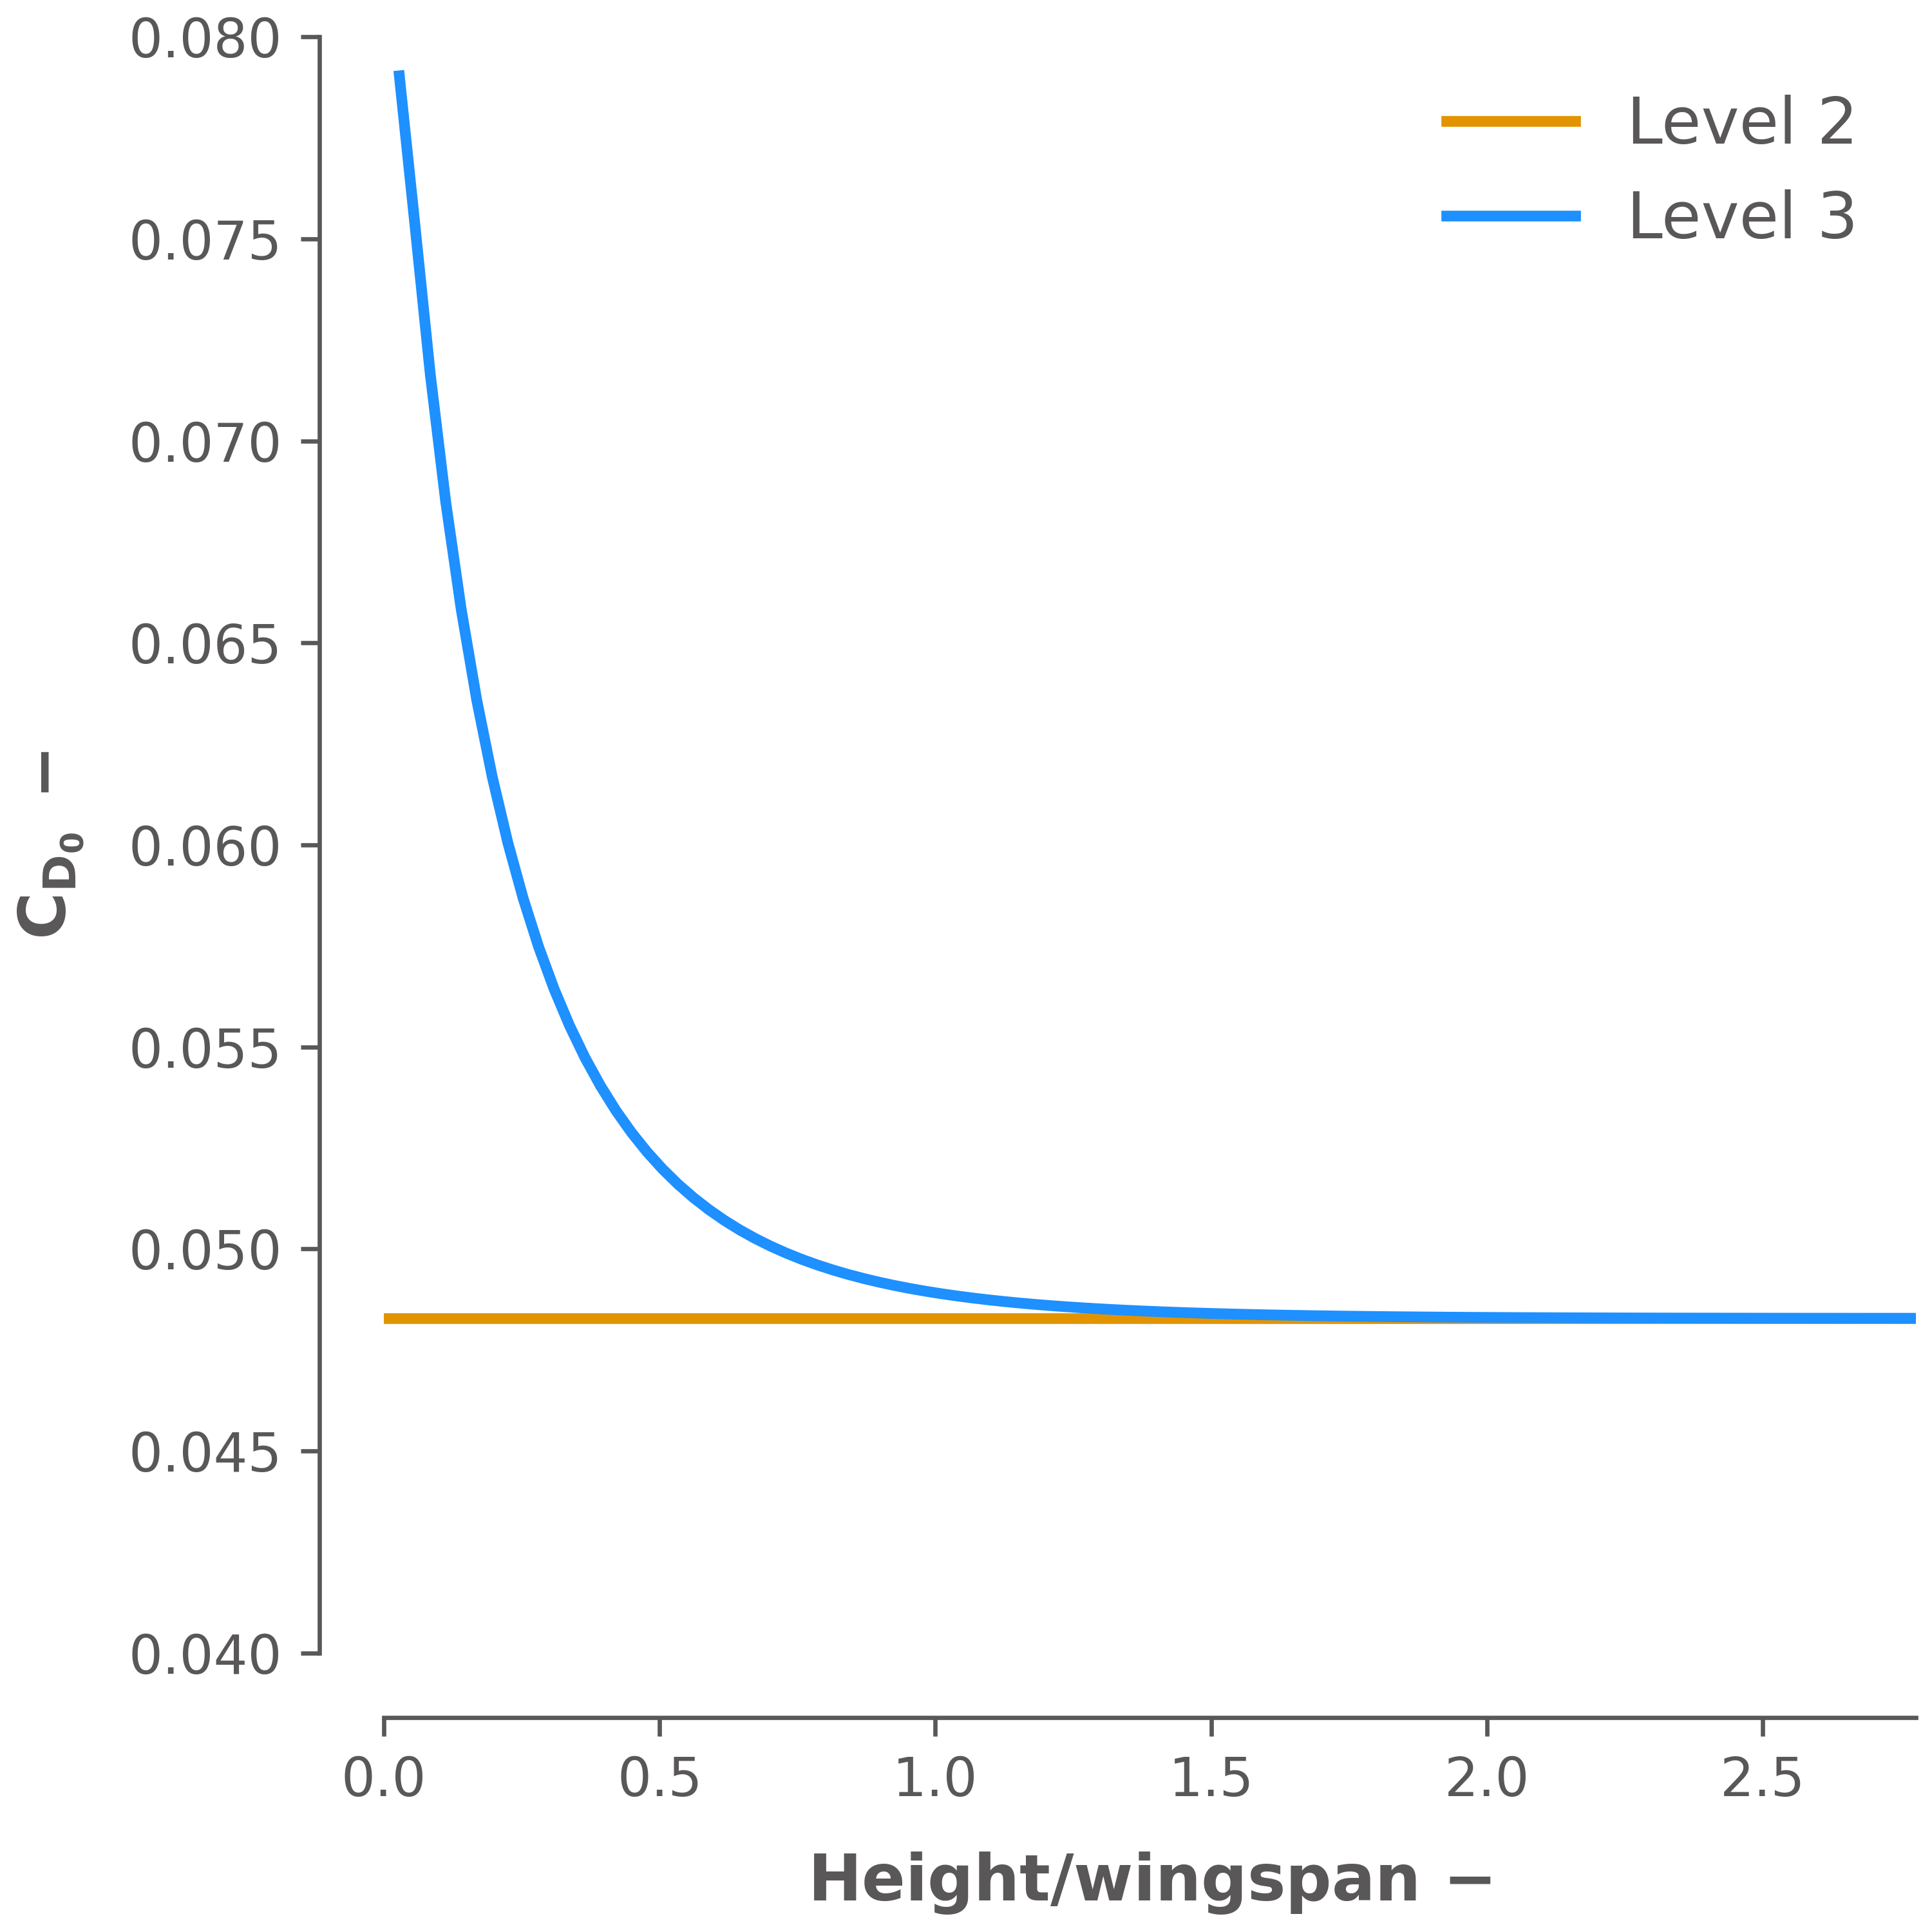
\includegraphics[width=\linewidth]{figures/CD2_CD3.png}
      \captionof{figure}{Comparison of level-II and level-III drag coefficients}
      \label{fig:drag_level2_3}
    \end{minipage}%
    \hfill
    \begin{minipage}{.48\textwidth}
      \centering
      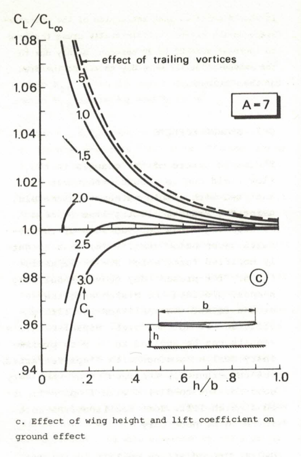
\includegraphics[width=\linewidth]{figures/cl2_cl3.png}
      \captionof{figure}{Comparison of level-II and level-III lift coefficients}
      \label{fig:lift_level2_3}
    \end{minipage}
\end{figure}

\section{Propeller Modelling}
% src-performance-newtonian-thrust_force.py\\
Modelling propeller performance is arguably one of the hardest tasks in take-off performance. Propeller modelling introdcues additional complexities since thrust is strongly dependent on advance ratio, blade pitch, and their fundamental connection to engine constraints. Furthermore, it is important to consider that the latter constraints differ for electrical and combustion engines. Electrical engines are not RPM constraint, and can thus operate at several rotational rate speeds. Furthermore, electrical engines are torque, and not power, constraint. Lastly, it is important to consider that propeller operating conditions can be different for electrical engines since there is no need to keep the engine spinning in ground idle conditions. The last effect complicating propeller modelling -- which is agnostic of the engine type -- is the lack of full-scale experimental data, and the abscence of accurate and inexpensive numerical models.\\
\\
Altogether, it means that propeller modelling is challenging. This sections aims to elaborate on the propeller mnodelling process for the take-off performance model. The section will start with stating the electrical engine propeller operating conditions. Afterwards, the two methods that were used for determining nominal propeller thrust will be given. Lastly, a determination of what the operative and inoperative propellers do for a continued and rejected take-off procedure is given.

\subsection{Propeller Operating Definitions}
Defining the propeller conditions is crucial to comply with CS25 regulations. After engine failure, during and accelerate-stop procedure, the operating engines must be set to a ground idle condition. Depending on whether the engine must maintain a certain RPM, or that zero power is a viable ground idle configuration, the propeller might generate a substantial amount of negative thrust. The propeller operating conditions are defined in \autoref{tab:propeller_oper_conditions}, with help of \autoref{fig:propeller_oper_conditions}. The latter shows a propeller performance map with several distinct points. The former then shows where each operating condition is located in the performance map.

\begin{table}[!ht]
    \caption{Propeller operating conditions}\label{tab:propeller_oper_conditions}
    \begin{tabular}{cc|ccccc}\\\hline \hline
        Propeller condition                         & Engine type       & Point     & Thrust    & Torque    & Pitch             & Rot rate \\ \hline
        \multirow{2}{*}{Failed, not feathered}      & Combustion        & E/F       & $T<0$     & $Q<0$     & $\beta_{min}$     & $n$ \\
                                                    & Electrical        & E/F       & $T<0$     & $Q<0$     & $\beta_{min}$     & $n$ \\
        \multirow{2}{*}{Failed, feathered}          & Combustion        & D1        & $T<0$     & $Q=0$     & $90$              & $n=0$ \\
                                                    & Electrical        & D1        & $T<0$     & $Q=0$     & $90$              & $n=0$ \\
        \multirow{2}{*}{Flight idle}                & Combustion        & A/B/C     & $T$       & $Q<0$     & $\beta_{min}$     & $n \neq 0$ \\
                                                    & Electrical        & A/B/C/D/E & $T$       & $Q$       & $\beta_{min}$     & $n \neq 0$ \\
        \multirow{2}{*}{Ground idle}                & Combustion        & A         & $T>0$     & $Q>0$     & $\beta_{min}$     & $n \neq 0$ \\
                                                    & Electrical        & A         & $T=0$     & $Q=0$     & $\beta_{min}$     & $n \neq 0$ \\
        \multirow{2}{*}{Ground fine, taxi}          & Combustion        & B         & $T=0$     & $Q>0$     & $\beta_{range}$   & $n \neq 0$ \\
                                                    & Electrical        & F         & $T=0$     & $Q=0$     & $\beta_{range}$   & $n \neq 0$ \\
        \multirow{2}{*}{Thrust reversal}            & Combustion        & C         & $T<0$     & $Q>0$     & $\beta_{rev}$     & $n \neq 0$ \\
                                                    & Electrical        & C         & $T<0$     & $Q>0$     & $\beta_{rev}$     & $n \neq 0$ \\
        \multirow{2}{*}{Nominal operation}          & Combustion        & C         & $T>0$     & $Q>0$     & $\beta$           & $n \neq 0$ \\
                                                    & Electrical        & C         & $T>0$     & $Q>0$     & $\beta$           & $n \neq 0$ \\
    \end{tabular}
\end{table}

\subsection{Nominal Propeller Thrust}\label{subsubsec:nominal_thrust_modelling}
As mentioned in the introduction; propeller thrust modelling is a complex issue. In the numerical modelling realm there's several options. The simplest is an actuator disk, with the most complex being a BEM with a vortex wake or particle method -- leaving unsteady 3D CFD out of consideration due to its computational overhead. An actuator disk gives thrust as a function of the efficiency, the freestream speed and the power input. You could vary the efficiency during the ground run, but those estimates would be hard to get without experimental data or high fidelity models of the propeller (and if you have that then actuator disk theory is superfluous). BEMT, or blade element momentum theory, is a proven and often validated method. However, the validation of BEMT often stops before it enters the low advance ratio regime, which is where most -- if not all -- of the take-off procedure takes place. And even the BEMT methods that work better during hover often have other limitations because they were developed for helicopter applications, who deal with much lower disk loadings.

All in all, none of these 3 methods offer a viable solution. Experimental data however can offer a solution. Little (to no) experimental data is available of full-scale propellers. However, NASA has published a series of papers on the propeller thrust, torque and power of several propellers. For the remainder of this section we will consider the $C_T$ and $C_P$ data of the 2-, 3- and 4-bladed NASA NACA5868-9 propellers.

The first issue with the experimental data is that after several attempts, it proved to be hard to find a well fitting surrogate function. The extracted NASA5868-9 data is shown in \autoref{fig:NASA5868_9_CT_CP_data}. It can be seen that the distance between blade pitch curves is not constant, nor monotonously decreasing. This non-monotonicity, makes it hard for a polynomial to approach the solution. Perhaps a different regression model would perform better, but for the time being this approach was discarded.

\begin{figure}[!ht]
    \centering
    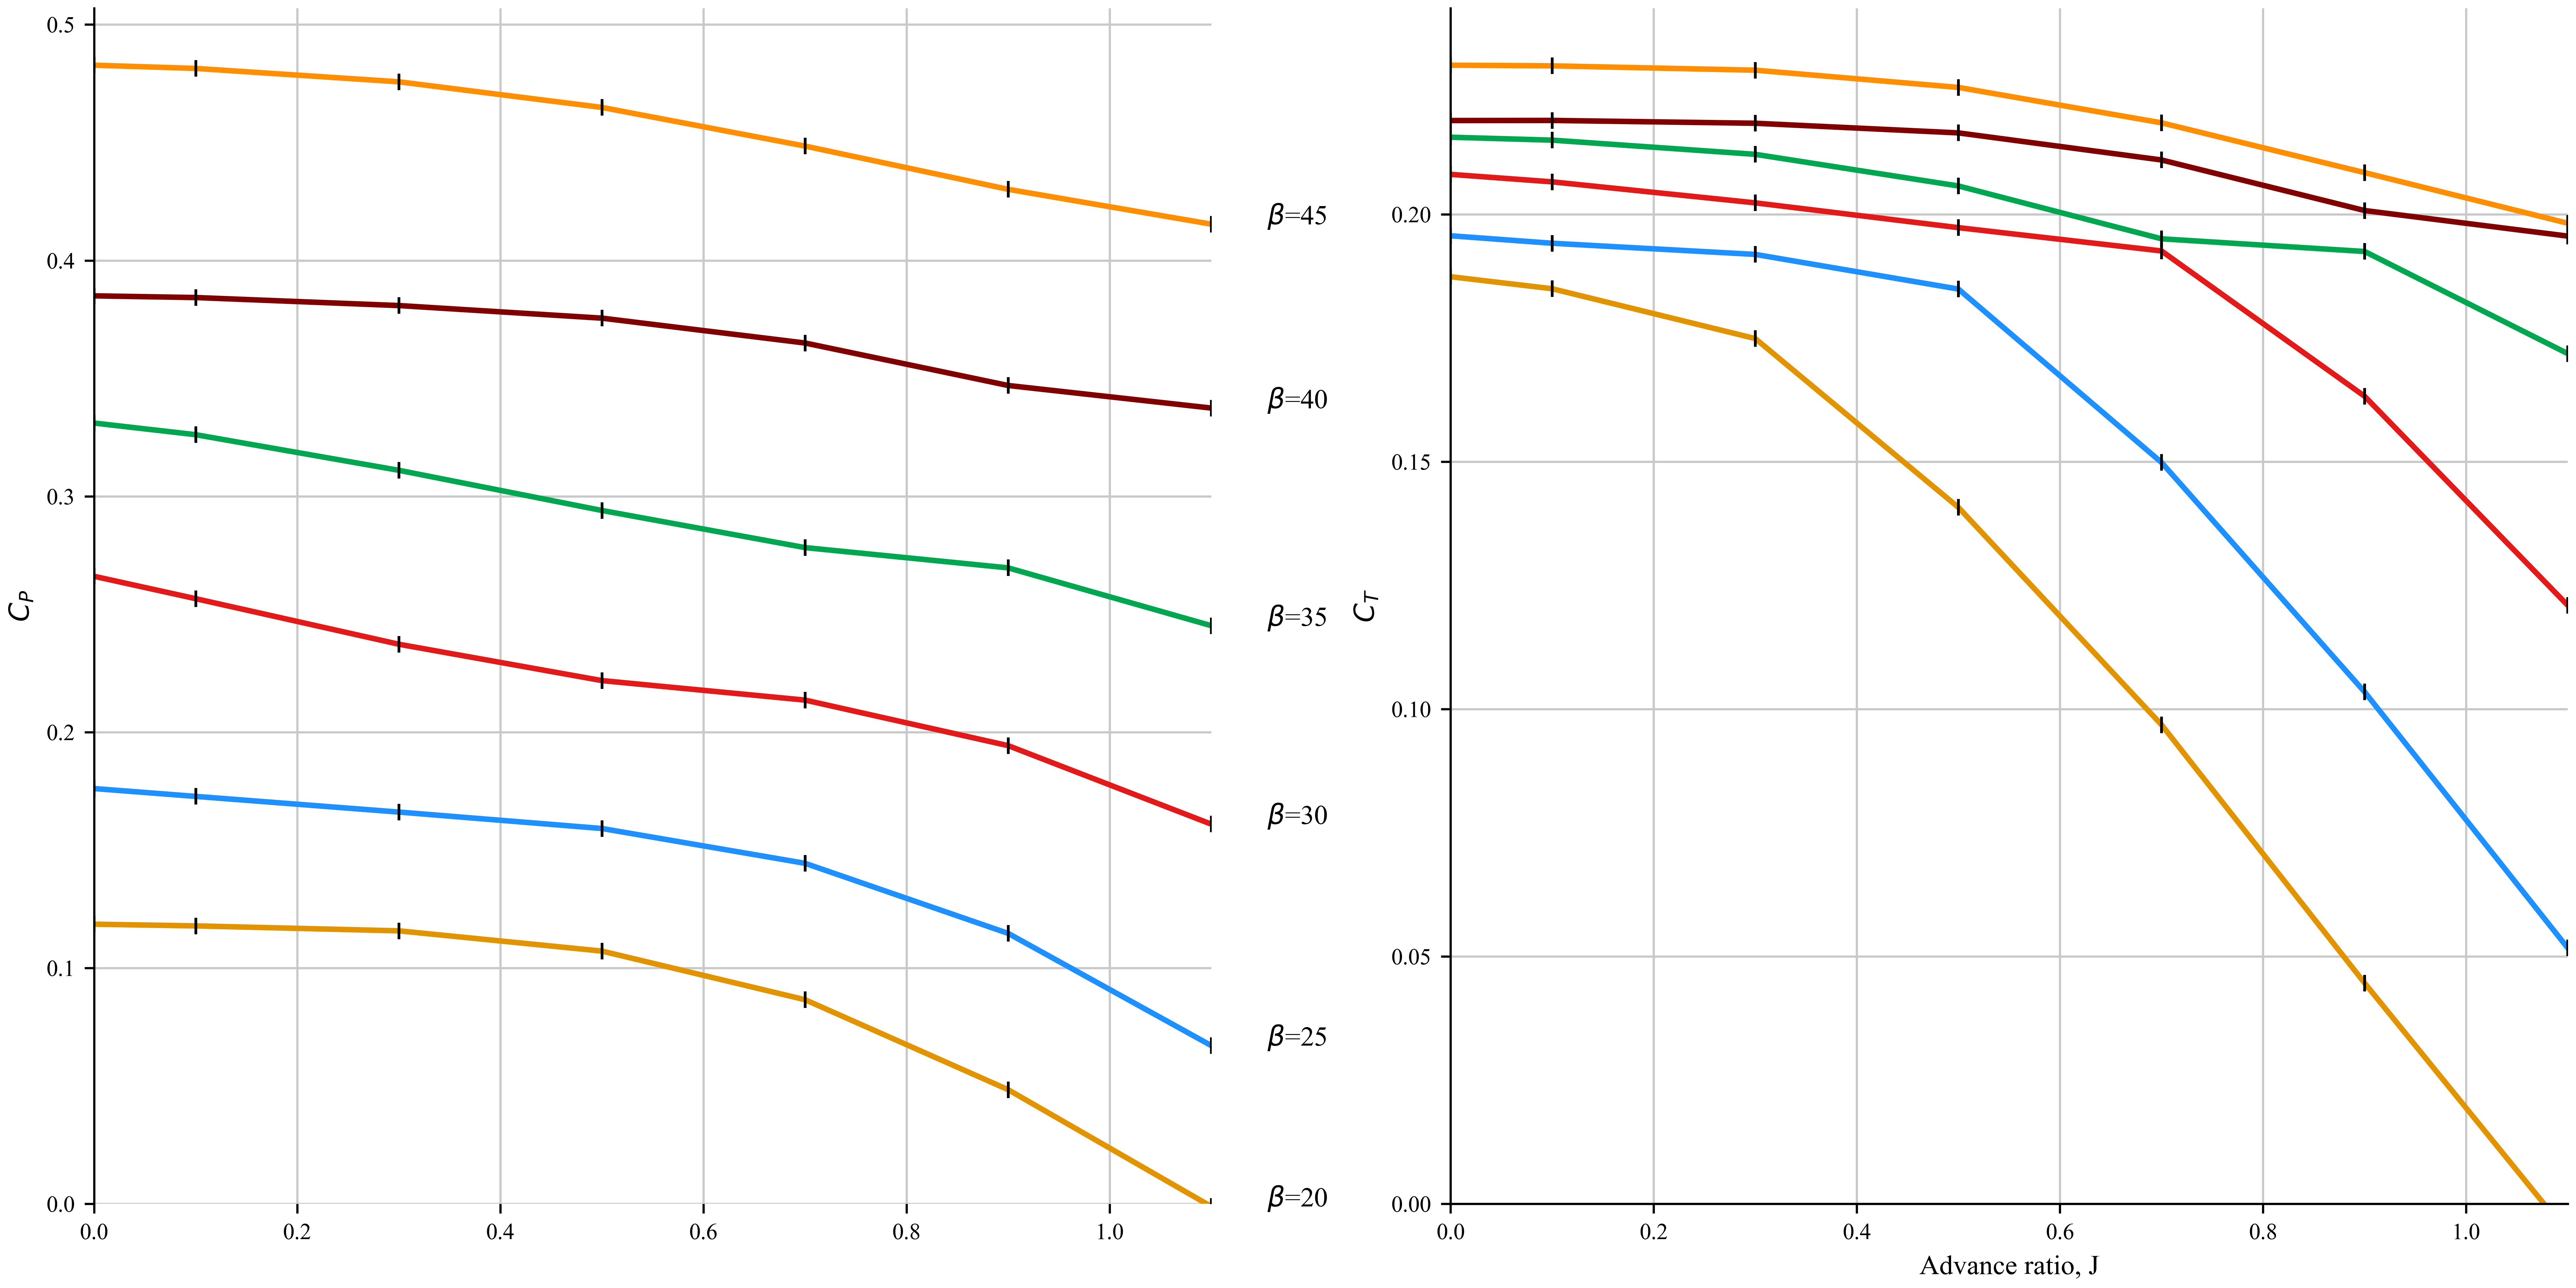
\includegraphics[width=0.5\linewidth]{figures/NASA5868_9_data.png}
    \caption{NASA5868-9 $C_T$ and $C_P$ data}\label{fig:NASA5868_9_CT_CP_data}
\end{figure}

The question remains; how do we `optimise' the NASA propeller for maximum thrust, given a maximum torque. The answer is Occam's razor: the simplest solution is often the best. Unfortunately, the simplest solution in this case did take a ton of time to implement: a 2D interpolation function. We start with an assumed maximum torque, and assume that \textit{the engine will always work at maximum torque during the take-off procedure}. Together with the rotational speed of the propeller, the maximum torque will give a maximum $C_P$. Assumption number 2 is that \textit{the propeller will always produce most thrust at the highest RPM}. This is a fair assumption since a potential higher $C_T$ value would have to compensate for the square of the loss in rotational rate. This is not impossible, but since the $C_T$ map is mostly linear until the blade stalls, it is assumed to be a safe assumption. With the $C_{P_\text{max}}$ and the $J$ (derived from the rotational rate and the given freestream velocity), we can find the propeller pitch. Afterwards, we can take the advance ratio and propeller pitch to the thrust performance map, which will give a $C_T$, and consequently thrust.

However, this is for a 4-bladed NASA 5868-9 propeller. The take-off performance tool needs to have the flexibility to vary the propeller design. Partly, we can already do this by varying the diameter and rotational speed. However, this would still leave us with a thrust coefficient that belongs to a 4 bladed propeller, where the E9X (currently) has 5 bladed propellers. To solve this issue we started to look into how well the 4- versus 5-bladed solutions scale to each other. In other words, can we multiply the 4 bladed $C_P$ and $C_T$ maps to get the 5-bladed performance map?

To assess the feasibility of this approach, 4 different scenarios were modelled: comparing thrust and power for a 2, 3 and 4 bladed propeller, at two pitch settings. This performance map comparison is shown in \autoref{fig:performance_map_comparison_nrblades}. In \autoref{fig:performance_map_comparison_nrblades} we see that there's a trend between the number of blades for each performance curve. The values near zero ($C_T$, $C_P$) cause some divergence of this factor at the higher advance ratios, which could also be augmented by experiment errors.

\begin{figure}[!ht]
    \centering
    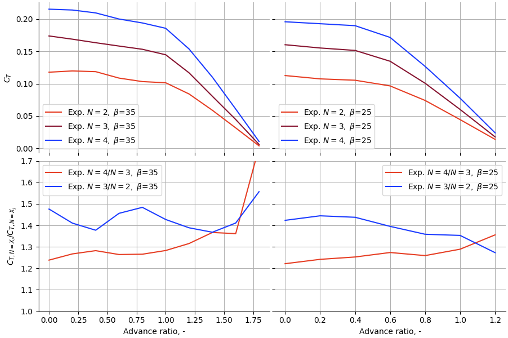
\includegraphics[width=0.5\linewidth]{figures/performancemap_comparison.png}
    \caption{Comparison of thrust and power performance for 2, 3 and 4 bladed propellers at $\beta=25,\;35$}
    \label{fig:performance_map_comparison_nrblades}
\end{figure}

The scaling factors for the 2 versus 3 versus 4 bladed propeller $C_T$ and $C_P$ values are given in \autoref{tab:nr_blades_comparison}. To arrive at the experimental fraction from the pure blade fraction, the latter values are multiplied by a newly defined loss factor. This factor embodies the phenomenon that multiplying the number of blades by factor $X$, does not multiply the thrust or power by a factor $X$. The scaling factor are fairly constant between the different pitch angles, which will be therefore assumed. The question now becomes, what is the loss factor of a 5 bladed propeller, versus a 4 bladed propeller. Generally, the loss factor seems to increase as the number of blades increases. To be conservative, an estimate is taken of the four values; 0.947 and 0.945 for the thrust and power performance maps, respectively. This equates to a scaling factor -- for the 4-bladed to the 5-bladed propeller -- of 1.184 and 1.181 for the thrust and power, respectively.

\begin{table}[!ht]
    \centering
    \caption{Propeller performance comparison for number of blades}\label{tab:nr_blades_comparison}
    \begin{tabular}{cccc}\\\hline \hline
        Blade pitch     & Nr. blades fraction   & $C_T$ loss factor     & $C_T$ experimental factor & $C_P$ loss factor     & $C_P$ experimental factor \\ \hline
        $25\deg$        & 4/3                   & 0.9412                & 1.250                     & 0.946                 & 1.261 \\
        $35\deg$        & 4/3                   & 0.9490                & 1.285                     & 0.971                 & 1.294 \\
        $25\deg$        & 3/2                   & 0.9375                & 1.412                     & 0.923                 & 1.384 \\
        $35\deg$        & 3/2                   & 0.964                 & 1.424                     & 0.939                 & 1.409 \\
    \end{tabular}
\end{table}

The thrust coefficient finding strategy remains the same, but now the thrust and power coefficients need ot be converted back and forth to use the 4-bladed values to obtain 5-bladed performance figures. To conclude, the current thrut model is based on experimental NASA data, scaled with an empirically factor to compensate for the number of blades.

\subsection{Post Engine Failure: Operative Propeller Thrust}
CS25 states that after engine failure, the remaining operating engines must be set to the ground idle configuration. We have defined ground idle to be a zero shaft power condition, where the blade pitch is at $\beta_{min}$. After engine failure, the propellers will be set to this pitch and the electrical engine will stop generating torque. As a consequence, the propeller will either accelerate or slow down, whilst extracting energy from the flow and decelerating the aircraft, until they reach an equilibrium position where the torque and power are zero. This process is shown in \autoref{fig:propeller_performance_postEF}.\\
\\
$\beta_{min}$ can be found by assessing the ground fine taxi operating condition through the following actions:
\begin{itemize}
    \item Assume a taxi velocity, $V_{taxi}=40;km/h,\;11.1\;m/s$
    \item Assume a taxi RPM, RPM=900
    \item 8 propellers must provide the thrust for the taxi condition. $D(V=11.1)=0.5 \rho V^2 S_{ref} C_{D_0}=15,130\;N$/propeller
    \item With the required thrust/propeller, and the RPM, we can find the required $C_T$: $C_T=15,130/(8 \rho n^2 D^4)=0.25$
    \item Remember to convert this to the $C_T$ for four blades, using the conversion factor discussed before: $C_{T,4 blades}=0.21$
    \item Look up in the NASA table, given in section \autoref{subsubsec:nominal_thrust_modelling}, at what pitch this thrust is given for $J=0.19$, $\beta_{min}=30\;deg$
\end{itemize}

This $\beta_{min}$ has a unique advance ratio at which $C_P=0$: $J=1.6$. We can see that the 4 and 3 bladed solutions coincide at their zero power point, so using this as a reference is a valid assumption. At $J=1.6$, the $C_T$ becomes $-0.018$, by linearly continuing the $C_T$ line. Converting this value back to a 5 bladed propeller we get $C_T=-0.021$. 

During the accelerate stop, the operating engines will be assumed to operate at this point and provide a constant $C_T=-0.021$, after engine failure. The RPM of the engines will vary however since the advance ratio remains constant and the aircraft slows down after engine failure. This way the negative thrust contibution of the engines will decrease with the aircraft velocity.

\subsection{Post Engine Failure: Inoperative Propeller Thrust}
After engine failure, the inoperative engine will generate neagtive thrust: drag. At two, three or even four engiend aircraft, this can be very significant for the continued take-off. However, as the number of propellers increases, the relative drag of the inoperative propeller decreases. Modelling the drag of an inoperative propeller depends on whether the propeller is feathered -- at 90 degrees pitch -- or whether the system is unfeathered. In the former case, the drag is about 8 times lower than for the unfeathered case. Raymer and Torenbeek both give methods for calculating the drag of a feathered propeller,

\begin{multicols}{2}
    \begin{equation}\label{eq:Raymer_featheredprop}
        C_{D_\text{inoperative}}=0.1 (\sigma A_{\text{prop}})/S_\text{ref} = 0.0005778,
    \end{equation}
    \begin{equation}\label{eq:Torenbeek_featheredprop}
        C_{D_\text{inoperative}}=0.00125 (B D_p^2)/S_\text{ref} = 0.0005064
    \end{equation}
\end{multicols}

Additionally, Raymer gives an estimate for the drag of an unfeathered propeller as well,

\begin{equation}\label{eq:Raymer_unfeatheredprop}
    C_{D_\text{inoperative}}=0.8 (\sigma A_{\text{prop}})/S_\text{ref} = 0.004051,
\end{equation}

where effectively the $0.1$ got replaced by a $0.8$. As can be seen in the E9X specific results above, the increase in drag is significant, compared to the $C_{D_0}$, which is 0.02, according to Torenbeek's estimate. Relatively this would mean a 5\%-20\% increase in drag. 

However, for the continued take-off scenario the inoperative propeller induced drag is negligible. Additionally, the E9X only loses 12.5\% of its thrust when an engine fails. The summation of the increase in profile drag, and loss in thrust therefore still remains small. For aircraft with fewer engines this drag penalty might be significant though.

\section{Miscellaneous Systems Modelling}
\subsection{Tire Modelling}
Furthermore, the roll friction coefficient is determined to be 0.02, as taken from Torenbeek~\cite{torenbeek2013synthesis}. The roll friction represents the imbalance between energy spent on the deforming of the tire: in other words, the backwards force to initially deform the tire is larger than the forward force when the tire goes back to its circular shape.\\
Wet surface\\
Gravel surface\\
Braking, anti-skid devices\\

\section{Take-Off Modelling Applications}

\subsection{All Engines Operative Take-Off}
The all engines operative, or zero engines inoperative, take-off is the simplest in terms of modelling since it doesn't require the system to change any further during the simulation. However, the all engines operative take-off is very important for sizing for aircraft with more than 4 engines. Obert suggests that aircraft with more than 4 engines have a less critical OEI sizing case because the loss in thrust due to one engine failing is inherently smaller. the E9X, with 8 propellers, is an extreme case of that. Even if EASA requires two engine failures, the loss in thrust will only be 25\%. The all engines opperative take-off distance must be multiplied by 1.15 according to CS25 rules, and then compared to the BFL, after which the longest becomes the critical take-off field length.

\subsection{Engine Inoperative After Engine Failure}

\subsection{Engine Operative Rejected Take-Off (Accelerate-Stop Distance)}

\subsection{Balanced Field Length}
The balanced field length (BFL) is a critical parameter in aviation that defines the minimum runway length required for an aircraft to safely accelerate to takeoff speed, undergo an engine failure at a predetermined point, and either continue the takeoff or abort and come to a stop within the remaining runway length. It represents an equilibrium between the aircraft's takeoff performance and its ability to safely stop in the event of an engine failure or other emergency during the initial phase of the takeoff roll. In essence, the balanced field length ensures that the aircraft can either commit to takeoff or safely abort the maneuver without exceeding the available runway length. Understanding and calculating the balanced field length is essential for flight crews, airport operators, and regulatory authorities to ensure the safety of flight operations and the efficient use of runway infrastructure.
